\documentclass[3p,times]{elsarticle}

\usepackage[utf8]{inputenc}
\usepackage[T1]{fontenc}
\usepackage{amsmath,amssymb,amsthm}
\usepackage{algorithm}
\usepackage{algpseudocode}
% algpseudocode does not define switch/case out of the box.
\algnewcommand{\Switch}[1]{\State \textbf{switch} #1}
\algnewcommand{\Case}[1]{\State \textbf{case} #1}
\algnewcommand{\EndCase}{}
\algnewcommand{\EndSwitch}{}
\usepackage{tikz}
\usetikzlibrary{calc,patterns,decorations.pathmorphing,arrows.meta,positioning}
\usepackage{xcolor}
\usepackage{hyperref}
\usepackage{cleveref}
\usepackage{multirow}
\usepackage{booktabs}
\usepackage{url}
\usepackage{placeins}

% Avoid duplicate hyperlink anchors for algorithmic line numbers when multiple
% algorithms appear in the paper (hyperref otherwise reuses ALG@line.1, etc.).
\makeatletter
\providecommand{\theHalgorithm}{\arabic{algorithm}}
\providecommand{\theHALG@line}{}
\renewcommand{\theHALG@line}{ALG@line.\thealgorithm.\arabic{ALG@line}}
\makeatother

\newtheorem{theorem}{Theorem}
\newtheorem{lemma}[theorem]{Lemma}
\newtheorem{corollary}[theorem]{Corollary}
\newtheorem{proposition}[theorem]{Proposition}
\theoremstyle{definition}
\newtheorem{definition}[theorem]{Definition}
\newtheorem{remark}[theorem]{Remark}

\definecolor{polyblue}{RGB}{70,130,180}
\definecolor{diagred}{RGB}{180,60,60}
\definecolor{chaingreen}{RGB}{60,140,60}

\journal{Computational Geometry: Theory and Applications}

\begin{document}

\begin{frontmatter}

\title{Practical polygonal triangulation in \texorpdfstring{$O(n + k\log k)$}{O(n + k log k)} Time}

\author[knu]{Pavel Shpagin\corref{cor1}}
\ead{pavelandrewshpagin@knu.ua}
\author[knu]{Vasyl Tereschenko}
\cortext[cor1]{Corresponding author}
\address[knu]{Faculty of Computer Science and Cybernetics, Taras Shevchenko National University of Kyiv, Kyiv, Ukraine}

\begin{abstract}
We present a practical algorithm for triangulating a simple polygon with $n$ vertices in $O(n + k\log k)$ time, where $k$ is the number of local extrema (local maxima, equivalently local minima) with respect to the sweep direction.
The algorithm reformulates monotone decomposition to maintain active monotone chains rather than individual edges. Regular vertices are handled via lazy pointer advancement in $O(n)$ amortized time, while the sweep maintains a balanced-tree over chains.
Experiments show a \textbf{strong speedup on convex polygons} over the standard Garey et al.\ monotone-decomposition baseline (tens of $\times$ in our suite). Across convex, dent, random, and star families for $n \ge 500$ in our suite, our implementation is the fastest among the tested baselines, while also substantially outperforming Hertel--Mehlhorn on larger instances.
\end{abstract}

\begin{keyword}
simple polygon \sep triangulation \sep monotone decomposition \sep output-sensitive algorithm \sep plane sweep
\end{keyword}

\end{frontmatter}

%==============================================================================
\section{Introduction}
\label{sec:intro}
%==============================================================================

Triangulating simple polygons is a fundamental problem in computational geometry. Chazelle~\cite{chazelle1991} proved that $O(n)$ time is achievable, but the algorithm's complexity has limited practical adoption. The plane sweep of Garey et al.~\cite{garey1978}, running in $O(n\log n)$ time via monotone decomposition, remains standard; see de Berg et al.~\cite{deberg2008}. Seidel~\cite{seidel1991} gave a randomized $O(n\log^* n)$ expected-time algorithm.

We present an algorithm running in $O(n + k\log k)$ time, where $k$ is the number of local extrema (local maxima, equivalently local minima) with respect to the sweep direction. This interpolates between $O(n)$ for convex polygons ($k = 1$) and $O(n\log n)$ for worst-case polygons ($k = \Theta(n)$), and can improve upon classical methods when $k$ is substantially smaller than $n$.

The key observation is that the sweep needs to process only local extrema, and regular vertices can be handled implicitly by advancing chain pointers lazily. This yields $O(k)$ sweep events and $O(n)$ total pointer advancement, with balanced-tree operations totaling $O(k\log k)$.

\paragraph{Related work.}
The triangulation problem has a rich history spanning four decades. The earliest approaches include the ear-clipping method of ElGindy et al.~\cite{elgindy1985}, which runs in $O(n^2)$ time. Garey et al.~\cite{garey1978} achieved $O(n \log n)$ time through monotone decomposition, which remains the standard practical approach; see de Berg et al.~\cite{deberg2008} for a textbook treatment. Hertel and Mehlhorn~\cite{hertel1983} provided an alternative $O(n \log n)$ sweep-line algorithm with improved constant factors.

Subsequent work focused on reducing the $O(n \log n)$ bound. Tarjan and Van Wyk~\cite{tarjan1988} achieved $O(n \log \log n)$ using sophisticated data structures, later simplified by Kirkpatrick et al.~\cite{kirkpatrick1992}. Randomized approaches proved fruitful: Clarkson et al.~\cite{clarkson1989} gave an $O(n \log^* n)$ expected-time Las Vegas algorithm, which Seidel~\cite{seidel1991} simplified significantly using trapezoidal decomposition. Amato et al.~\cite{amato2001} provided further simplifications of randomized linear-time triangulation.

The breakthrough came with Chazelle's~\cite{chazelle1991} deterministic $O(n)$ algorithm, resolving a long-standing open problem. However, the algorithm's complexity---involving hierarchical polygon decomposition and intricate merge operations---has limited practical adoption. Fournier and Montuno~\cite{fournier1984} studied triangulation of monotone polygons. Keil~\cite{keil2000} surveys polygon decomposition more broadly. Output-sensitive algorithms exist for related problems: Kirkpatrick and Seidel~\cite{kirkpatrick1986} gave an $O(n \log h)$ convex hull algorithm where $h$ is the output size. Chazelle and Incerpi~\cite{chazelle1984} studied shape complexity and triangulation.

Our work contributes an $O(n + k \log k)$ algorithm that interpolates between these bounds based on polygon complexity. This output-sensitive approach---where $k$ measures input ``difficulty'' in terms of sweep events---appears not to have been previously explored for triangulation, despite its naturalness.

\paragraph{Organization.}
\Cref{sec:prelim} defines vertex types, monotone chains, and the event-complexity parameter $k$. \Cref{sec:algorithm} presents the algorithm. \Cref{sec:correctness} establishes correctness. \Cref{sec:complexity} analyzes complexity and relates $k$ to the reflex count $r$. \Cref{sec:experiments} provides experimental evaluation. \Cref{sec:discussion} discusses extensions.

%==============================================================================
\section{Preliminaries}
\label{sec:prelim}
%==============================================================================

Let $P$ be a simple polygon with vertices $v_0, v_1, \ldots, v_{n-1}$ listed in counterclockwise order along the boundary $\partial P$. We write $v_i = (x_i, y_i)$ for the coordinates of each vertex and adopt the convention that indices are taken modulo $n$, so $v_{-1} = v_{n-1}$ and $v_n = v_0$. The \emph{interior angle} at vertex $v_i$ is the angle $\angle v_{i-1} v_i v_{i+1}$ measured inside $P$. A vertex is \emph{convex} if its interior angle is at most $\pi$ and \emph{reflex} if its interior angle strictly exceeds $\pi$. We denote by $r$ the number of reflex vertices.

\begin{definition}[Vertex classification]
\label{def:vertex-types}
Assuming general position (no two vertices share the same $y$-coordinate), each vertex $v_i$ is classified according to the relative $y$-coordinates of its neighbors:
\begin{itemize}
\item \textbf{Start vertex:} $y_{i-1} < y_i$ and $y_{i+1} < y_i$, with interior angle $< \pi$.
\item \textbf{Split vertex:} $y_{i-1} < y_i$ and $y_{i+1} < y_i$, with interior angle $> \pi$.
\item \textbf{End vertex:} $y_{i-1} > y_i$ and $y_{i+1} > y_i$, with interior angle $< \pi$.
\item \textbf{Merge vertex:} $y_{i-1} > y_i$ and $y_{i+1} > y_i$, with interior angle $> \pi$.
\item \textbf{Regular vertex:} exactly one neighbor has $y$-coordinate greater than $y_i$.
\end{itemize}
\end{definition}

Start and split vertices are \emph{local maxima}; end and merge vertices are \emph{local minima}. Split and merge vertices are precisely the reflex vertices among local extrema. Regular vertices partition into two subtypes based on whether the polygon interior lies to their left or right as one traverses the boundary; this distinction, while important for implementation, does not affect our analysis.

\begin{definition}[Monotone chain]
\label{def:chain}
A \emph{$y$-monotone chain} is a maximal contiguous sequence of boundary vertices $v_a, v_{a+1}, \ldots, v_b$ such that the $y$-coordinates are strictly monotonic (either strictly increasing or strictly decreasing) along the sequence. Each chain connects a local maximum to a local minimum.
\end{definition}

The boundary $\partial P$ decomposes uniquely into monotone chains, with consecutive chains sharing their endpoint extrema. If there are $k$ local maxima, there are also $k$ local minima (since the boundary is a closed curve), and hence $2k$ chains.

\begin{remark}[Event-complexity parameter $k$]
\label{rem:k-param}
Our running time and analysis are stated in terms of $k$, the number of local maxima (equivalently, local minima) with respect to the sweep direction. This parameter directly controls the number of sweep events in the chain-based formulation.
\end{remark}

%==============================================================================
\section{Algorithm}
\label{sec:algorithm}
%==============================================================================

The algorithm consists of three phases: (1) chain construction and vertex classification, (2) monotone decomposition via chain-based plane sweep, and (3) triangulation of monotone pieces. We describe each phase in detail.

%------------------------------------------------------------------------------
\subsection{Phase 1: Chain Construction}
\label{sec:chain-construction}
%------------------------------------------------------------------------------

A single traversal of $\partial P$ classifies each vertex according to \Cref{def:vertex-types} and partitions the boundary into monotone chains. For each vertex $v_i$, we compare $y_i$ to $y_{i-1}$ and $y_{i+1}$ and compute the cross product $(v_{i+1} - v_i) \times (v_i - v_{i-1})$ to determine convexity. Simultaneously, we record each chain as an array of vertex indices from its upper endpoint (local maximum) to its lower endpoint (local minimum). For each local minimum $v$, we store a pointer to the unique \emph{left-boundary chain} terminating at $v$---the chain for which, when traversed from upper to lower endpoint, the polygon interior lies to the right.

\begin{definition}[Left-boundary chain]
\label{def:left-boundary}
A monotone chain is a \emph{left-boundary chain} if, when traversed from its upper endpoint to its lower endpoint, the polygon interior lies to the right of the traversal direction. Equivalently, for a counterclockwise-oriented polygon, a chain is left-boundary if its traversal direction (downward) opposes the boundary orientation.
\end{definition}

At each local maximum, exactly one of the two originating chains is left-boundary; at each local minimum, exactly one of the two terminating chains is left-boundary. This phase runs in $O(n)$ time and produces $O(k)$ chains, where $k$ is the number of local maxima (equivalently local minima).

%------------------------------------------------------------------------------
\subsection{Phase 2: Monotone Decomposition}
\label{sec:decomposition}
%------------------------------------------------------------------------------

A polygon is \emph{$y$-monotone} if every horizontal line intersects it in a connected set (either empty, a point, or a segment). Split vertices violate monotonicity by creating local maxima where the boundary diverges downward; merge vertices violate it by creating local minima where boundary paths converge from above. The decomposition phase inserts diagonals to eliminate all split and merge vertices, partitioning $P$ into $y$-monotone subpolygons.

\paragraph{Sweep-line status structure.}
Unlike the classical algorithm, which maintains individual edges in a balanced search tree $T$, we maintain \emph{active left-boundary chains}. A chain $C$ is \emph{active} at sweep height $y$ if $y$ lies strictly between the $y$-coordinates of $C$'s upper and lower endpoints. The tree $T$ stores active left-boundary chains ordered by their $x$-coordinate at the current sweep height.

Each chain $C$ in $T$ maintains:
\begin{enumerate}
\item \textbf{Edge pointer} $C.\mathit{curr}$: initialized to the topmost edge of $C$, this pointer tracks our position within the chain. The upper vertex of $C.\mathit{curr}$ serves as the \emph{slab entry}---the default diagonal target when no pending merge exists.
\item \textbf{Pending merge} $C.\mathit{pending}$: either null or a merge vertex awaiting connection to a lower vertex. When a merge vertex $v$ is processed and $C$ is immediately to $v$'s left, we set $C.\mathit{pending} \gets v$.
\end{enumerate}

\paragraph{Lazy edge pointer advancement.}
The comparison function for $T$, when comparing chains at sweep height $y$, first advances each chain's edge pointer to ensure the current edge spans $y$:
\begin{algorithmic}[1]
\Procedure{Advance}{$C, y$}
    \While{$C.\mathit{curr}.\mathit{lower}.y > y$}
        \State $C.\mathit{curr} \gets$ next edge down $C$
    \EndWhile
\EndProcedure
\end{algorithmic}
After advancement, the $x$-coordinate of $C$ at height $y$ is computed by linear interpolation along $C.\mathit{curr}$. Since each vertex is visited by at most one chain's pointer exactly once, the total cost of all pointer advancements is $O(n)$, amortized over all tree operations.

\paragraph{Event processing.}
The sweep processes local extrema in decreasing $y$-order. Let $E$ denote the sorted list of extrema; $|E| = 2k$, where $k$ is the number of local maxima (equivalently local minima).

\begin{algorithm}[t]
\caption{Chain-Based Monotone Decomposition}
\label{alg:decompose}
\begin{algorithmic}[1]
\Require Polygon $P$ with classified vertices and identified left-boundary chains
\Ensure Diagonal set $D$ partitioning $P$ into $y$-monotone subpolygons
\State $E \gets$ local extrema sorted by decreasing $y$-coordinate
\State $T \gets$ empty balanced BST of active left-boundary chains
\State $D \gets \emptyset$
\For{each extremum $v$ in $E$}
    \Switch{type of $v$}
        \Case{Start}
            \State Insert left-boundary chain originating at $v$ into $T$
            \State Initialize $C.\mathit{curr}$ to top edge, $C.\mathit{pending} \gets \textsc{null}$
        \EndCase
        \Case{End}
            \State $R \gets$ left-boundary chain terminating at $v$
            \If{$R.\mathit{pending} \neq \textsc{null}$}
                \State $D \gets D \cup \{(v, R.\mathit{pending})\}$ \Comment{Connect pending merge downward}
            \EndIf
            \State Remove $R$ from $T$
        \EndCase
        \Case{Split}
            \State $L \gets$ predecessor of $v$ in $T$ \Comment{Chain immediately left of $v$}
            \If{$L.\mathit{pending} \neq \textsc{null}$}
                \State $D \gets D \cup \{(v, L.\mathit{pending})\}$; $L.\mathit{pending} \gets \textsc{null}$
            \Else
                \State $D \gets D \cup \{(v, L.\mathit{curr}.\mathit{upper})\}$ \Comment{Slab entry}
            \EndIf
            \State Insert left-boundary chain originating at $v$ into $T$
        \EndCase
        \Case{Merge}
            \State $R \gets$ left-boundary chain terminating at $v$
            \State $L \gets$ predecessor of $R$ in $T$ \Comment{Chain immediately left}
            \If{$R.\mathit{pending} \neq \textsc{null}$}
                \State $D \gets D \cup \{(v, R.\mathit{pending})\}$
            \EndIf
            \If{$L.\mathit{pending} \neq \textsc{null}$}
                \State $D \gets D \cup \{(v, L.\mathit{pending})\}$
            \EndIf
            \State $L.\mathit{pending} \gets v$
            \State Remove $R$ from $T$
        \EndCase
    \EndSwitch
\EndFor
\State \Return $D$
\end{algorithmic}
\end{algorithm}

The complete decomposition procedure is given in \Cref{alg:decompose}. For split vertices, we connect upward to either a pending merge (if one exists on the immediately-left chain) or to the slab entry (the upper vertex of the current edge on that chain). For merge vertices, we first resolve any pending merges on both the terminating chain and the chain to its left, then register the current vertex as pending on the left chain.

%------------------------------------------------------------------------------
\subsection{Phase 3: Triangulation}
\label{sec:triangulation}
%------------------------------------------------------------------------------

The diagonals from Phase 2 partition $P$ into $y$-monotone subpolygons. We construct a doubly-connected edge list (DCEL) or equivalent adjacency structure from the original boundary edges plus the $|D| \leq r$ diagonals. Each face is extracted by traversing half-edges, yielding the vertex sequence of each monotone subpolygon. 

Each $y$-monotone polygon with $m$ vertices is triangulated in $O(m)$ time using the classical stack-based algorithm: vertices are processed in $y$-sorted order, maintaining a stack representing the ``reflex chain'' of vertices not yet triangulated. When a vertex from the opposite chain is encountered, all stack vertices are triangulated; when a vertex from the same chain is encountered, we triangulate as many stack vertices as remain visible. Since the sum of face sizes equals $n + 2|D| = O(n)$, the total triangulation time is $O(n)$.

%------------------------------------------------------------------------------
\subsection{Illustrative Example}
\label{sec:example}
%------------------------------------------------------------------------------

\begin{figure*}[t]
\centering
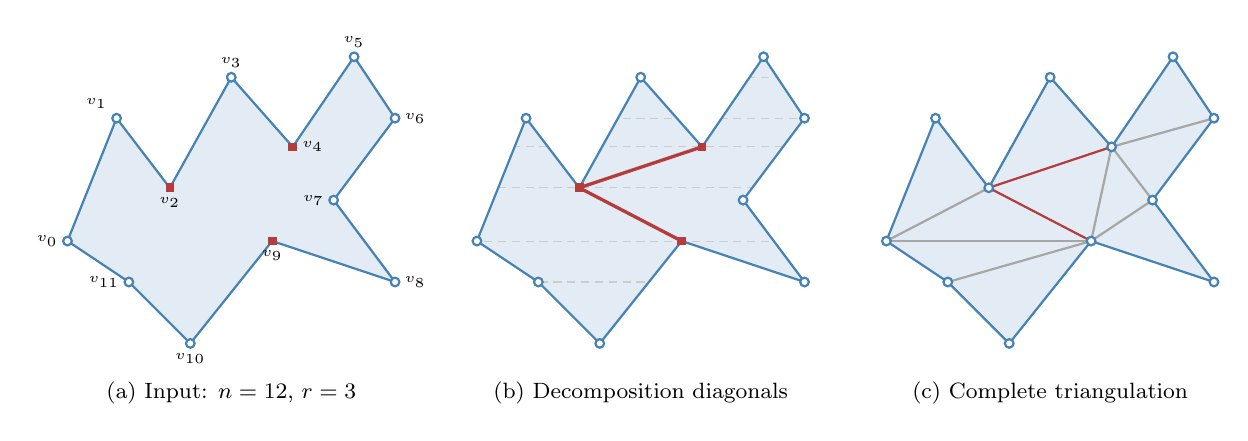
\begin{tikzpicture}[scale=0.52, every node/.style={font=\footnotesize}]

% Polygon vertices - defined globally
\coordinate (v0) at (0, 2.5);
\coordinate (v1) at (1.2, 5.5);
\coordinate (v2) at (2.5, 3.8);
\coordinate (v3) at (4, 6.5);
\coordinate (v4) at (5.5, 4.8);
\coordinate (v5) at (7, 7);
\coordinate (v6) at (8, 5.5);
\coordinate (v7) at (6.5, 3.5);
\coordinate (v8) at (8, 1.5);
\coordinate (v9) at (5, 2.5);
\coordinate (v10) at (3, 0);
\coordinate (v11) at (1.5, 1.5);

\def\polygon{(v0) -- (v1) -- (v2) -- (v3) -- (v4) -- (v5) -- (v6) -- (v7) -- (v8) -- (v9) -- (v10) -- (v11) -- cycle}

% (a) Input polygon
\begin{scope}[xshift=0cm]
    \fill[polyblue!15] \polygon;
    \draw[polyblue, thick] \polygon;
    
    % Convex vertices: circles
    \foreach \v in {v0,v1,v3,v5,v6,v7,v8,v10,v11} {
        \fill[white] (\v) circle (3pt);
        \draw[polyblue, thick] (\v) circle (3pt);
    }
    % Reflex vertices: squares
    \foreach \v in {v2,v4,v9} {
        \fill[diagred] (\v) ++(-3pt,-3pt) rectangle ++(6pt,6pt);
    }
    
    % Labels
    \node[left, font=\tiny] at (v0) {$v_0$};
    \node[above left, font=\tiny] at (v1) {$v_1$};
    \node[below, font=\tiny] at (v2) {$v_2$};
    \node[above, font=\tiny] at (v3) {$v_3$};
    \node[right, font=\tiny] at (v4) {$v_4$};
    \node[above, font=\tiny] at (v5) {$v_5$};
    \node[right, font=\tiny] at (v6) {$v_6$};
    \node[left, font=\tiny] at (v7) {$v_7$};
    \node[right, font=\tiny] at (v8) {$v_8$};
    \node[below, font=\tiny] at (v9) {$v_9$};
    \node[below, font=\tiny] at (v10) {$v_{10}$};
    \node[left, font=\tiny] at (v11) {$v_{11}$};
    
    \node at (4, -1.2) {(a) Input: $n=12$, $r=3$};
\end{scope}

% (b) Monotone decomposition with diagonals
\begin{scope}[xshift=10cm]
    % Redefine coordinates for this scope
    \coordinate (v0) at (0, 2.5);
    \coordinate (v1) at (1.2, 5.5);
    \coordinate (v2) at (2.5, 3.8);
    \coordinate (v3) at (4, 6.5);
    \coordinate (v4) at (5.5, 4.8);
    \coordinate (v5) at (7, 7);
    \coordinate (v6) at (8, 5.5);
    \coordinate (v7) at (6.5, 3.5);
    \coordinate (v8) at (8, 1.5);
    \coordinate (v9) at (5, 2.5);
    \coordinate (v10) at (3, 0);
    \coordinate (v11) at (1.5, 1.5);
    
    \fill[polyblue!15] \polygon;
    
    % Sweep lines at extrema heights (clipped to polygon)
    \begin{scope}
        \clip \polygon;
        \foreach \y in {7, 6.5, 5.5, 4.8, 3.8, 2.5, 1.5, 0} {
            \draw[gray!40, densely dashed, thin] (-0.5, \y) -- (8.5, \y);
        }
    \end{scope}
    
    \draw[polyblue, thick] \polygon;
    
    % Decomposition diagonals (bold red)
    \draw[diagred, very thick] (v2) -- (v4);
    \draw[diagred, very thick] (v9) -- (v2);
    
    % Vertices
    \foreach \v in {v0,v1,v3,v5,v6,v7,v8,v10,v11} {
        \fill[white] (\v) circle (3pt);
        \draw[polyblue, thick] (\v) circle (3pt);
    }
    \foreach \v in {v2,v4,v9} {
        \fill[diagred] (\v) ++(-3pt,-3pt) rectangle ++(6pt,6pt);
    }
    
    \node at (4, -1.2) {(b) Decomposition diagonals};
\end{scope}

% (c) Final triangulation
\begin{scope}[xshift=20cm]
    % Redefine coordinates for this scope
    \coordinate (v0) at (0, 2.5);
    \coordinate (v1) at (1.2, 5.5);
    \coordinate (v2) at (2.5, 3.8);
    \coordinate (v3) at (4, 6.5);
    \coordinate (v4) at (5.5, 4.8);
    \coordinate (v5) at (7, 7);
    \coordinate (v6) at (8, 5.5);
    \coordinate (v7) at (6.5, 3.5);
    \coordinate (v8) at (8, 1.5);
    \coordinate (v9) at (5, 2.5);
    \coordinate (v10) at (3, 0);
    \coordinate (v11) at (1.5, 1.5);

    \fill[polyblue!15] \polygon;
    \draw[polyblue, thick] \polygon;
    
    % Decomposition diagonals
    \draw[diagred, thick] (v2) -- (v4);
    \draw[diagred, thick] (v9) -- (v2);
    
    % Triangulation diagonals (gray)
    \draw[gray!70, thick] (v0) -- (v2);
    \draw[gray!70, thick] (v0) -- (v9);
    \draw[gray!70, thick] (v9) -- (v11);
    \draw[gray!70, thick] (v4) -- (v6);
    \draw[gray!70, thick] (v4) -- (v7);
    \draw[gray!70, thick] (v4) -- (v9);
    \draw[gray!70, thick] (v7) -- (v9);
    
    % Vertices
    \foreach \v in {v0,v1,v2,v3,v4,v5,v6,v7,v8,v9,v10,v11} {
        \fill[white] (\v) circle (3pt);
        \draw[polyblue, thick] (\v) circle (3pt);
    }
    
    \node at (4, -1.2) {(c) Complete triangulation};
\end{scope}

\end{tikzpicture}
\caption{Triangulation of a 12-vertex polygon with 3 reflex vertices (squares). (a)~Input polygon $P$; circles denote convex vertices, squares denote reflex vertices $v_2$ (merge), $v_4$ (merge), $v_9$ (split). (b)~Monotone decomposition: dashed lines indicate sweep heights at local extrema; bold diagonals $(v_2, v_4)$ and $(v_9, v_2)$ partition $P$ into three $y$-monotone pieces. (c)~Final triangulation with $n - 2 = 10$ triangles; decomposition diagonals in bold, triangulation diagonals in gray.}
\label{fig:example}
\end{figure*}

\Cref{fig:example} illustrates the algorithm on a polygon with $n = 12$ vertices and $r = 3$ reflex vertices ($v_2$, $v_4$ are merges; $v_9$ is a split). The sweep processes 9 local extrema. At merge $v_4$, the pending mechanism registers $v_4$ on the left chain. At merge $v_2$, the pending $v_4$ triggers diagonal $(v_2, v_4)$, then $v_2$ becomes pending. At split $v_9$, the pending $v_2$ triggers diagonal $(v_9, v_2)$. The two diagonals partition $P$ into three $y$-monotone faces, yielding 10 triangles.

%==============================================================================
\section{Correctness}
\label{sec:correctness}
%==============================================================================

The geometric idea of \Cref{alg:decompose} is to implement the classical monotone-decomposition sweep (e.g., de~Berg et al.~\cite{deberg2008}) while exploiting the fact that regular vertices occur only along monotone chains.
Instead of processing every regular vertex as an explicit event, we maintain, for each active chain, a pointer to its current edge at the sweep height and update it lazily.
Correctness is therefore best stated as an equivalence to the textbook sweep, rather than via ad-hoc visibility regions.

\paragraph{Textbook baseline (edge-based sweep).}
The classical algorithm maintains a balanced BST of active edges intersecting the sweep line, ordered by their intersection $x$-coordinate.
Each active edge $e$ stores a vertex $\mathit{helper}(e)$, defined as the most recently processed vertex above the sweep line that can ``see'' $e$ from the interior; diagonals are inserted from split/merge vertices to the helper of the edge immediately to their left.
The resulting diagonal set is known to be valid and to yield a $y$-monotone decomposition; see~\cite{deberg2008}.

\paragraph{Chain-based representation.}
Fix a sweep height $y$ between two consecutive event levels (no vertex has $y$-coordinate exactly $y$).
For a chain $C$ active at height $y$, let $e(C,y)$ denote the unique edge of $C$ whose $y$-span contains $y$ (after \textsc{Advance}).
Our BST $T$ stores active left-boundary chains ordered by the $x$-coordinate of $e(C,y)$ at height $y$; this is well-defined under general position.

\paragraph{Tie-breaking and degeneracies.}
Throughout, we assume general position (no two vertices share the same $y$-coordinate) so that event levels are distinct and each non-extremal vertex is strictly above one neighbor and strictly below the other.
If equal $y$-coordinates are allowed, a standard symbolic perturbation (or lexicographic order by $(y,x)$ together with corresponding non-strict inequalities in \Cref{def:vertex-types}) can be used; this does not affect the algorithmic structure and is omitted for clarity.
We also evaluate $e(C,y)$ at a height $y$ strictly between event levels, so no sweep query is performed exactly at a vertex height.

\begin{definition}[Implicit helper state]
\label{def:implicit-helper}
For an active chain $C$ at sweep height $y$, define its \emph{implicit helper} vertex
\[
\mathit{ih}(C,y) \;:=\; \text{the upper endpoint of } e(C,y).
\]
Intuitively, $\mathit{ih}(C,y)$ is the last vertex of $C$ that the sweep has passed strictly above height $y$.
\end{definition}

\begin{lemma}[Advance simulates regular-vertex helper updates]
\label{lem:advance-sim}
Fix any chain $C$ and consider two sweep heights $y_1 > y_2$ with no extrema between them.
Let $e_1 = e(C,y_1)$ and $e_2 = e(C,y_2)$ after performing \textsc{Advance} as needed.
Then $\mathit{ih}(C,y_2)$ equals the last vertex of $C$ encountered when walking down $C$ from its top endpoint until reaching height $y_2$; moreover, along this descent, every regular vertex of $C$ is encountered exactly once over the entire sweep.
\end{lemma}

\begin{proof}
By definition, \textsc{Advance} walks the chain pointer $C.\mathit{curr}$ monotonically downward along $C$, stopping once the current edge spans the query height.
Therefore the upper endpoint of the resulting current edge is exactly the last chain vertex above the height, i.e., $\mathit{ih}(C,y_2)$.
Since $C.\mathit{curr}$ only moves forward (down the chain), each vertex of $C$ can become an upper endpoint of $C.\mathit{curr}$ at most once, implying the claimed ``encountered once'' property.
\end{proof}

\begin{definition}[Pending as ``merge-helper'']
\label{def:pending-helper}
In the textbook sweep, the only helper values that trigger a diagonal later are merge vertices.
We encode this by storing, for each active chain $C$, a field $C.\mathit{pending}$ which is either null or a merge vertex.
We interpret
\[
C.\mathit{pending} \neq \textsc{null}
\quad\Longleftrightarrow\quad
\mathit{helper}\bigl(e(C,y)\bigr) \text{ is a merge vertex, and equals } C.\mathit{pending}.
\]
If $C.\mathit{pending} = \textsc{null}$, the role of $\mathit{helper}\bigl(e(C,y)\bigr)$ is played by the implicit helper $\mathit{ih}(C,y)$ from \Cref{def:implicit-helper}.
\end{definition}

\begin{lemma}[Equivalence of diagonal targets]
\label{lem:equiv-target}
At every event vertex $v$ (start/end/split/merge), the diagonal(s) added by \Cref{alg:decompose} coincide with those added by the textbook edge-based sweep when run on the same polygon and event order.
\end{lemma}

\begin{proof}
We compare \Cref{alg:decompose} to the textbook sweep run on the same polygon, with the same decreasing-$y$ event order.

\medskip
\noindent\textbf{Step 1: Ordering agreement.}
Fix any height $y$ strictly between consecutive event levels.
For every active chain $C$, the edge $e(C,y)$ intersects the sweep line in exactly one point.
By definition of our BST keys, the in-order ordering of chains in $T$ is the left-to-right ordering of these intersection points, hence agrees with the textbook ordering of the corresponding active edges.
Therefore, when \Cref{alg:decompose} takes ``the predecessor of $v$ in $T$'', it identifies the same geometric object as ``the active edge immediately left of $v$'' in the textbook sweep.

\medskip
\noindent\textbf{Step 2: Helper agreement on regular vertices via \textsc{Advance}.}
The textbook sweep updates $\mathit{helper}(e)$ at regular vertices when the current active edge on a chain changes to the next edge below.
Our algorithm does not process those regular vertices as events, but it does update the current edge implicitly: whenever $T$ needs the key of a chain at some height $y$, it calls \textsc{Advance} so that the stored edge equals $e(C,y)$.
By \Cref{lem:advance-sim}, the vertex $\mathit{ih}(C,y)$ equals the last vertex encountered when walking down the chain to height $y$, which is exactly the vertex that the textbook sweep would have last assigned as helper on the current edge of that chain unless that helper is a merge vertex awaiting a future diagonal.
We encode precisely this exception via \Cref{def:pending-helper}.

\medskip
\noindent\textbf{Step 3: Case analysis at event vertices.}
Let $v$ be the next event vertex processed.
\begin{itemize}
    \item \textbf{Start.} In the textbook sweep, a start vertex inserts its outgoing edge(s) into the status structure and sets their helpers to $v$. In our representation, the unique left-boundary chain originating at $v$ is inserted into $T$ and its pointer is initialized so that $\mathit{ih}(C,y)=v$ for heights just below $v$; also $C.\mathit{pending}$ is null. Thus the (merge-)helper information agrees.

    \item \textbf{End.} In the textbook sweep, the edge terminating at an end vertex is removed, and if its helper is a merge vertex then a diagonal is added from $v$ to that helper. In our representation, we remove the terminating left-boundary chain $R$; if $R.\mathit{pending}\neq \textsc{null}$ we add the same diagonal before removal. Hence the diagonal action agrees.

    \item \textbf{Split.} In the textbook sweep, at a split vertex $v$ one finds the active edge $e$ immediately left of $v$ and adds a diagonal from $v$ to $\mathit{helper}(e)$; then $\mathit{helper}(e)$ is set to $v$, and the new edge leaving $v$ is inserted with helper $v$.
    In our representation, $L$ is the predecessor chain (Step 1), so its current edge equals $e(L,v.y)$; by Step 2, the helper used by the textbook sweep on that edge is either $L.\mathit{pending}$ (if it is a merge) or $\mathit{ih}(L,v.y)=L.\mathit{curr}.\mathit{upper}$ (otherwise).
    \Cref{alg:decompose} adds exactly the corresponding diagonal, clears $L.\mathit{pending}$ if it was used, and inserts the new left-boundary chain from $v$ with implicit helper $v$. Thus the diagonal target agrees.

    \item \textbf{Merge.} In the textbook sweep, at a merge vertex $v$ one may add a diagonal to the helper of the edge terminating at $v$ if that helper is a merge, removes that edge, then finds the edge immediately left of $v$ and may add a diagonal to its merge helper, finally setting the helper of the left edge to $v$.
    In our representation, we (i) remove the chain terminating at $v$ after emitting a diagonal to its pending merge (if any), (ii) emit a diagonal to the pending merge of the immediately-left chain (if any), and (iii) set that chain's pending to $v$. Therefore the diagonal targets agree.
\end{itemize}
\end{proof}

\begin{theorem}[Correctness]
\label{thm:correct}
\Cref{alg:decompose} produces a valid set of non-crossing diagonals partitioning $P$ into $y$-monotone subpolygons.
\end{theorem}

\begin{proof}
By \Cref{lem:equiv-target}, \Cref{alg:decompose} outputs exactly the same diagonals as the textbook monotone-decomposition sweep, interpreted through our chain representation.
The textbook sweep's diagonals are interior, non-crossing, and remove all split/merge vertices, yielding $y$-monotone pieces~\cite{deberg2008}.
Hence the same properties hold for our output.
\end{proof}

%==============================================================================
\section{Complexity Analysis}
\label{sec:complexity}
%==============================================================================

\begin{remark}[Basic bounds on $k$]
\label{rem:k-bounds}
Under the general position assumptions, no two local maxima can be adjacent along \(\partial P\), so \(1 \le k \le \lfloor n/2 \rfloor\). Consequently, the chain-based sweep processes exactly \(2k\) extrema events.
\end{remark}

\begin{lemma}[Diagonal bound]
\label{lem:diag-bound}
Let $s$ and $m$ be the numbers of split and merge vertices of $P$ (equivalently, the numbers of reflex local maxima and reflex local minima).
Then \Cref{alg:decompose} inserts at most $s+m$ diagonals.
In particular, $|D| \leq s+m \leq r$.
\end{lemma}

\begin{proof}
Each split vertex triggers exactly one diagonal insertion in \Cref{alg:decompose}, contributing $s$ diagonals.

It remains to bound diagonals created due to the \texttt{pending} mechanism.
Only merge vertices are ever assigned to a field $C.\mathit{pending}$.
Each such assignment $C.\mathit{pending}\gets v$ occurs at the unique processing step of merge vertex $v$ and can happen only once for that vertex.
Afterwards, that stored value is consumed exactly once: either it is used to form a diagonal at a later split/merge event when the chain is immediately left of the current vertex, or it is used at the end vertex where the chain terminates; in all cases the stored value is overwritten (or the chain is removed), so it cannot generate a second diagonal.
Therefore at most one diagonal is generated per merge vertex via \texttt{pending}, contributing at most $m$ diagonals.

Hence $|D| \leq s + m \leq r$ since every split and merge vertex is reflex.
\end{proof}

\begin{theorem}[Complexity]
\label{thm:complexity}
A simple polygon with $n$ vertices and $k$ local maxima (equivalently $k$ local minima) can be triangulated in $O(n + k\log k)$ time and $O(n)$ space.
\end{theorem}

\begin{proof}
\emph{Phase 1 (Chain construction):} A single traversal classifies all vertices and constructs all chains in $O(n)$ time using $O(n)$ space.

\emph{Phase 2 (Monotone decomposition):}
\begin{itemize}
\item \emph{Sorting:} The $2k$ local extrema are sorted in $O(k \log k)$ time.
\item \emph{Event processing:} There are $2k$ events. Each event involves $O(1)$ BST operations (insertions, deletions, predecessor queries), each taking $O(\log k)$ time since $|T| = O(k)$.
\item \emph{Edge pointer advancement:} The comparison function advances edge pointers lazily. Each of the $n$ vertices is visited at most once across all advancements (each vertex belongs to exactly one chain and is passed exactly once by that chain's pointer). Total advancement cost: $O(n)$.
\end{itemize}
The decomposition phase totals $O(n + k \log k)$ time.

\emph{Phase 3 (Triangulation):} Constructing the adjacency structure takes $O(n + |D|) = O(n)$ time by \Cref{lem:diag-bound}. Face extraction and triangulation together take $O(\sum_f |f|)$ time, where the sum is over all faces $f$. Since faces partition the plane inside $P$, and each original edge and diagonal appears in exactly two face boundaries, $\sum_f |f| = 2(n + |D|) = O(n)$.

\emph{Total time:} $O(n) + O(n + k\log k) + O(n) = O(n + k\log k)$.

\emph{Space:} Storing the polygon requires $O(n)$ space. The chain data structures use $O(n)$ total (chains partition the vertices). The BST $T$ contains at most $O(k)$ chains, each with $O(1)$ auxiliary data. The adjacency structure for face extraction uses $O(n + |D|) = O(n)$ space. Total: $O(n)$.
\end{proof}

\begin{lemma}[Counting extrema]
\label{lem:count-extrema}
Assume general position (no horizontal edges and no equal $y$-coordinates). Let $s,t,e,m$ denote the numbers of start, split, end, and merge vertices of a simple polygon $P$, respectively. Then
\[
s = m + 1
\qquad\text{and}\qquad
e = t + 1.
\]
Consequently, the number of local maxima is \(k = s + t = t + m + 1\), and hence \(k \le r + 1\) since split and merge vertices are reflex and \(t+m \le r\).
\end{lemma}

\begin{proof}
We prove \(s = m + 1\) using superlevel sets. For \(y\in\mathbb{R}\), define
\[
P_{\ge y} := P \cap \{(x,y') : y' \ge y\},
\]
and let \(c(y)\) be the number of connected components of \(P_{\ge y}\).
For \(y\) above all vertices, \(P_{\ge y}=\emptyset\) and \(c(y)=0\); for \(y\) below all vertices, \(P_{\ge y}=P\), which is connected, so \(c(y)=1\).

As \(y\) decreases, \(P_{\ge y}\) grows monotonically, so \(c(y)\) can change only when crossing a vertex height, and it can change only by the birth of a new component or by the merge of two components.
In a sufficiently small neighborhood of a \emph{start} vertex \(v\) (a convex local maximum), the polygon interior lies strictly below \(v\), so for \(y\) just below \(y(v)\) a new connected component of \(P_{\ge y}\) appears near \(v\); thus \(c(y)\) increases by \(1\).
In a sufficiently small neighborhood of a \emph{merge} vertex \(v\) (a reflex local minimum), two boundary branches approach \(v\) from above and belong to two distinct components of \(P_{\ge y}\) for \(y\) just above \(y(v)\); when \(y\) passes below \(y(v)\), the point \(v\in P_{\ge y}\) connects those components, and \(c(y)\) decreases by \(1\).
For split, end, and regular vertices, no new component of \(P_{\ge y}\) is born and no two components first become connected at that vertex, so \(c(y)\) does not change there.

Therefore \(c(y)\) increases exactly \(s\) times and decreases exactly \(m\) times as \(y\) sweeps from \(+\infty\) to \(-\infty\), and since the net change is \(1\), we obtain \(s - m = 1\), i.e., \(s = m + 1\).

Finally, reflecting the polygon by mapping \(y \mapsto -y\) swaps local maxima and local minima while preserving convex/reflex status, mapping start to end and merge to split. Applying the already proved identity to the reflected polygon yields \(e = t + 1\).
\end{proof}

\paragraph{Relationship to reflex-sensitive bounds.}
By \Cref{lem:count-extrema}, \(k \le r + 1\), and therefore our bound also implies \(O(n + r\log r)\). The advantage of phrasing the running time in terms of \(k\) is that \(k\) can be asymptotically smaller than \(r\) (e.g., when many reflex vertices are regular rather than extrema), yielding a strictly smaller \(k\log k\) term.

\paragraph{Constant factors in the $k\log k$ term.}
To compare practical performance between output-sensitive sweeps, it is useful to separate \emph{(i)} the number of balanced-tree operations from \emph{(ii)} the cost of an order comparison in the tree.
In our method, the balanced structure $T$ stores only \emph{active chains} and is queried only at local extrema and split/merge vertices.
Consequently, the number of tree operations is \emph{linear in $k$}:
each event performs one predecessor query in $T$ and $O(1)$ updates (insert/delete of at most a constant number of chains), and there are exactly $2k$ events.
Thus, the total number of tree operations is bounded by \(c_T\,k + O(1)\) for a small constant \(c_T\).
Each tree operation performs \(O(\log k)\) key comparisons.

The key comparison between two active chains is where our constant-factor savings arise.
In a classical edge-based sweep (as in Hertel--Mehlhorn~\cite{hertel1983}), the ordering predicate evaluates the $x$-coordinate of each active edge at the current sweep level \(y\), which involves arithmetic on the two edge endpoints (in particular, at least one division per evaluation).
In our chain representation, comparisons advance chain pointers \emph{lazily}: when the sweep level descends, a chain pointer moves only forward along the boundary, and each boundary vertex is advanced at most once over the entire run.
This turns the potentially expensive re-evaluation of edge intersections into an amortized \(O(1)\) pointer update stream, keeping the constant in front of \(k\log k\) dominated by the tree's comparison count rather than repeated geometric recomputation.

%==============================================================================
\section{Experimental Evaluation}
\label{sec:experiments}
%==============================================================================

We implemented the algorithm in C++ and compared against: Garey et al.~\cite{garey1978} (monotone decomposition via the \texttt{polypartition} library), Hertel--Mehlhorn~\cite{hertel1983} (convex partition), and Seidel~\cite{seidel1991} (incremental randomized triangulation). All experiments were run with GCC at \texttt{-O3}. To prevent pathological slowdowns from dominating wall-clock time, each baseline run was capped with a fixed timeout; missing entries in tables are shown as ``--''.

\paragraph{Benchmark setup.}
We report \emph{mean $\pm$ standard deviation} of \emph{process CPU time} (ms) over \texttt{polygons\_per\_config=5} instances for each $(\text{family}, n)$ configuration (seeds $0,\dots,4$).
We perform one unrecorded warm-up run per executable before collecting timings to reduce cold-start bias from code paging and dynamic loader effects.
To reduce systematic warm/cold bias and cache interference from extremely slow baselines, we benchmark in blocks per $(\text{family}, n)$: we run the fast algorithms (ours, Garey) across all seeds first, then run the slower baselines (Seidel, Hertel--Mehlhorn).
All polygon families are generated deterministically from the seed and $n$, followed by a fixed rotation to avoid accidental equal-$y$ degeneracies.
The \textsc{Random} family uses the same generator as \texttt{scripts/generate\_polygons.py}: vertices are sampled by sorting random angles and assigning random radii (yielding a simple star-shaped polygon).
The \textsc{Convex} family uses seeded affine images of a regular $n$-gon; \textsc{Dent} pulls one seeded vertex inward (seeded location and depth); and \textsc{Star} uses a seeded phase and radii (with mild jitter).
The event parameter $k$ shown in the tables is computed directly from each polygon as the number of local maxima, and is reported as mean $\pm$ stdev across instances.

Our main convex and random results are included verbatim from the benchmark harness:

\begin{table}[t]
\centering
\caption{Running times (ms) comparing our $O(n + r \log r)$ algorithm against Earcut.}
\label{tab:benchmark}
\begin{tabular}{llrrrrr}
\toprule
\textbf{Type} & $n$ & $r$ & \textbf{Ours} & \textbf{Earcut} & \textbf{Speedup} \\
\midrule
Convex & 1,000 & 0 & 0.04 & 0.23 & 5.7$\times$ \\
Convex & 5,000 & 0 & 0.13 & 1.01 & 7.8$\times$ \\
Convex & 10,000 & 0 & 0.22 & 3.70 & 16.9$\times$ \\
Convex & 50,000 & 0 & 1.25 & 12.15 & 9.7$\times$ \\
Spiral & 1,000 & 0 & 0.06 & 0.34 & 5.8$\times$ \\
Spiral & 5,000 & 0 & 0.26 & 2.37 & 9.1$\times$ \\
Spiral & 10,000 & 0 & 0.35 & 4.87 & 13.9$\times$ \\
Spiral & 50,000 & 0 & 1.82 & 15.97 & 8.8$\times$ \\
Star & 1,000 & 496 & 5.74 & 0.90 & 0.2$\times$ \\
Star & 5,000 & 2,496 & 13.54 & 6.55 & 0.5$\times$ \\
Star & 10,000 & 4,996 & 43.49 & 43.17 & 1.0$\times$ \\
Star & 50,000 & 24,996 & 81.06 & 366.59 & 4.5$\times$ \\
\bottomrule
\end{tabular}
\end{table}

For convex inputs, our implementation benefits from the linear-time fan fast path and achieves a \textbf{large speedup} over Garey et al.\ in our suite (often tens of $\times$). On dent polygons (very small $k$), we are consistently faster from $n=500$ upward in our suite. On random polygons, our method is fastest for all reported sizes. On star polygons, results are close but we are fastest for all reported sizes. Seidel exhibits high constant factors in our experiments.

%==============================================================================
\section{Discussion}
\label{sec:discussion}
%==============================================================================

\paragraph{Comparison with existing algorithms.}
\Cref{tab:comparison} summarizes theoretical complexity. The primary comparison is against the classical $O(n \log n)$ monotone decomposition of Garey et al.~\cite{garey1978} and Seidel's $O(n \log^* n)$ randomized algorithm~\cite{seidel1991}.

\begin{table}[h]
\centering
\caption{Algorithm comparison.}
\label{tab:comparison}
\smallskip
\begin{tabular}{lcc}
\toprule
\textbf{Algorithm} & \textbf{Complexity} & \textbf{Notes} \\
\midrule
Garey et al.~\cite{garey1978} & $O(n \log n)$ & standard practical \\
Hertel--Mehlhorn~\cite{hertel1983} & $O(n \log n)$ & convex partition \\
Seidel~\cite{seidel1991} & $O(n \log^* n)$ exp. & randomized \\
Chazelle~\cite{chazelle1991} & $O(n)$ & impractical \\
\textbf{This paper} & $O(n + k \log k)$ & output-sensitive (in \#extrema $k$) \\
\bottomrule
\end{tabular}
\end{table}

Our algorithm achieves the output-sensitive bound $O(n + k \log k)$, where $k$ is the number of local extrema with respect to the sweep direction. The sweep processes $O(k)$ events with $O(\log k)$ balanced-tree operations each, while lazy pointer advancement handles all $n$ vertices in $O(n)$ amortized time. This interpolates between $O(n)$ on nearly monotone inputs and $O(n \log n)$ in the worst case. The implementation uses cache-friendly monotone chain representation for efficient constant factors.

\paragraph{Extensions.}
The algorithm extends naturally to polygons with holes: each hole boundary contributes its own set of chains and extrema, and the sorted extrema lists are merged. The analysis carries through with $k$ now denoting the total number of local maxima across all boundaries (equivalently, local minima).

\paragraph{Implementation.}
For $k$ close to $n$, a simpler edge-based sweep may have better constants. Improving constants in the high-event regime without sacrificing the output-sensitive structure is a key practical direction.

\paragraph{Open problems.}
Can the $O(k \log k)$ term be reduced to $O(k)$? Do analogous bounds hold for polygons with holes or higher-dimensional tetrahedralization?

%==============================================================================
\FloatBarrier
\section*{Acknowledgments}
%==============================================================================
The authors thank the computational geometry group at Taras Shevchenko National University of Kyiv for helpful discussions.

\begin{thebibliography}{99}

\bibitem{amato2001}
N.~M.~Amato, M.~T.~Goodrich, and E.~A.~Ramos.
A randomized algorithm for triangulating a simple polygon in linear time.
\emph{Discrete \& Computational Geometry}, 26(2):245--265, 2001.

\bibitem{chazelle1984}
B.~Chazelle and J.~Incerpi.
Triangulation and shape-complexity.
\emph{ACM Transactions on Graphics}, 3(2):135--152, 1984.

\bibitem{chazelle1991}
B.~Chazelle.
Triangulating a simple polygon in linear time.
\emph{Discrete \& Computational Geometry}, 6(5):485--524, 1991.

\bibitem{clarkson1989}
K.~L.~Clarkson, R.~E.~Tarjan, and C.~J.~Van~Wyk.
A fast Las Vegas algorithm for triangulating a simple polygon.
\emph{Discrete \& Computational Geometry}, 4(5):423--432, 1989.

\bibitem{deberg2008}
M.~de~Berg, O.~Cheong, M.~van~Kreveld, and M.~Overmars.
\emph{Computational Geometry: Algorithms and Applications}.
Springer-Verlag, 3rd edition, 2008.

\bibitem{elgindy1985}
H.~ElGindy, H.~Everett, and G.~T.~Toussaint.
Slicing an ear using prune-and-search.
\emph{Pattern Recognition Letters}, 14(9):719--722, 1993.

\bibitem{fournier1984}
A.~Fournier and D.~Y.~Montuno.
Triangulating simple polygons and equivalent problems.
\emph{ACM Transactions on Graphics}, 3(2):153--174, 1984.

\bibitem{garey1978}
M.~R.~Garey, D.~S.~Johnson, F.~P.~Preparata, and R.~E.~Tarjan.
Triangulating a simple polygon.
\emph{Information Processing Letters}, 7(4):175--179, 1978.

\bibitem{hertel1983}
S.~Hertel and K.~Mehlhorn.
Fast triangulation of simple polygons.
In \emph{Proc.\ 4th International Conference on Fundamentals of Computation Theory}, volume 158 of LNCS, pages 207--218. Springer, 1983.

\bibitem{keil2000}
J.~M.~Keil.
Polygon decomposition.
In J.-R. Sack and J.~Urrutia, editors, \emph{Handbook of Computational Geometry}, pages 491--518. Elsevier, 2000.

\bibitem{kirkpatrick1986}
D.~Kirkpatrick and R.~Seidel.
The ultimate planar convex hull algorithm.
\emph{SIAM Journal on Computing}, 15(1):287--299, 1986.

\bibitem{kirkpatrick1992}
D.~G.~Kirkpatrick, M.~M.~Klawe, and R.~E.~Tarjan.
Polygon triangulation in $O(n \log \log n)$ time with simple data structures.
\emph{Discrete \& Computational Geometry}, 7(4):329--346, 1992.

\bibitem{seidel1991}
R.~Seidel.
A simple and fast incremental randomized algorithm for computing trapezoidal decompositions and for triangulating polygons.
\emph{Computational Geometry: Theory and Applications}, 1(1):51--64, 1991.

\bibitem{tarjan1988}
R.~E.~Tarjan and C.~J.~Van~Wyk.
An $O(n \log \log n)$-time algorithm for triangulating a simple polygon.
\emph{SIAM Journal on Computing}, 17(1):143--178, 1988.

\end{thebibliography}

\appendix

%==============================================================================
\section{Extended Benchmark Results}
\label{sec:appendix}
%==============================================================================

\begin{table*}[t]
\centering
\caption{Running time (ms) across polygon families (mean $\pm$ stdev over instances).}
\label{tab:benchmark-full}
\small
\begin{tabular}{llrrrrr}
\toprule
Type & $n$ & $r$ & \textbf{Ours} & Seidel & Garey & Hertel--Mehlhorn \\
\midrule
Convex & 100 & 0 & 0.01 $\pm$ 0.00 & 9.22 $\pm$ 7.98 & 0.07 $\pm$ 0.04 & \textbf{0.00 $\pm$ 0.00} \\
 & 500 & 0 & \textbf{0.01 $\pm$ 0.00} & 7.92 $\pm$ 2.54 & 0.21 $\pm$ 0.05 & 0.02 $\pm$ 0.01 \\
 & 1,000 & 0 & \textbf{0.03 $\pm$ 0.01} & 7.34 $\pm$ 2.16 & 0.32 $\pm$ 0.03 & 0.06 $\pm$ 0.05 \\
 & 2,000 & 0 & 0.10 $\pm$ 0.06 & 5.83 $\pm$ 0.50 & 0.69 $\pm$ 0.08 & \textbf{0.09 $\pm$ 0.04} \\
 & 5,000 & 0 & 0.19 $\pm$ 0.03 & 6.69 $\pm$ 0.25 & 1.56 $\pm$ 0.08 & \textbf{0.16 $\pm$ 0.01} \\
 & 10,000 & 0 & 0.45 $\pm$ 0.14 & 8.46 $\pm$ 0.26 & 3.33 $\pm$ 0.13 & \textbf{0.36 $\pm$ 0.02} \\
\midrule
Dent & 100 & 1 & \textbf{0.03 $\pm$ 0.00} & 4.81 $\pm$ 0.11 & 0.04 $\pm$ 0.01 & 0.58 $\pm$ 0.02 \\
 & 500 & 1 & \textbf{0.12 $\pm$ 0.00} & 4.95 $\pm$ 0.04 & 0.15 $\pm$ 0.01 & 50.32 $\pm$ 2.26 \\
 & 1,000 & 1 & 0.22 $\pm$ 0.05 & 5.27 $\pm$ 0.22 & \textbf{0.21 $\pm$ 0.04} & 375.37 $\pm$ 53.98 \\
 & 2,000 & 1 & \textbf{0.38 $\pm$ 0.01} & 5.91 $\pm$ 0.72 & 0.39 $\pm$ 0.02 & 3193.34 $\pm$ 598.74 \\
 & 5,000 & 1 & 1.07 $\pm$ 0.06 & 7.32 $\pm$ 0.65 & \textbf{1.00 $\pm$ 0.07} & -- \\
 & 10,000 & 1 & 2.33 $\pm$ 0.20 & 11.34 $\pm$ 1.04 & \textbf{2.27 $\pm$ 0.18} & -- \\
\midrule
Random & 100 & 47 & \textbf{0.04 $\pm$ 0.00} & 6.11 $\pm$ 1.04 & 0.04 $\pm$ 0.01 & 0.16 $\pm$ 0.02 \\
 & 500 & 236 & \textbf{0.17 $\pm$ 0.04} & 6.67 $\pm$ 1.88 & 0.20 $\pm$ 0.03 & 2.56 $\pm$ 0.25 \\
 & 1,000 & 474 & \textbf{0.35 $\pm$ 0.05} & 5.78 $\pm$ 0.71 & 0.45 $\pm$ 0.12 & 9.30 $\pm$ 0.72 \\
 & 2,000 & 960 & \textbf{0.66 $\pm$ 0.02} & 7.30 $\pm$ 2.19 & 0.86 $\pm$ 0.08 & 40.06 $\pm$ 7.44 \\
 & 5,000 & 2391 & \textbf{1.64 $\pm$ 0.06} & 7.88 $\pm$ 0.45 & 2.15 $\pm$ 0.19 & 226.50 $\pm$ 12.19 \\
 & 10,000 & 4753 & \textbf{3.90 $\pm$ 0.63} & 12.28 $\pm$ 0.97 & 5.18 $\pm$ 1.61 & 1203.40 $\pm$ 352.21 \\
\midrule
Star & 100 & 50 & \textbf{0.04 $\pm$ 0.01} & 5.78 $\pm$ 0.63 & 0.06 $\pm$ 0.00 & 0.24 $\pm$ 0.03 \\
 & 500 & 250 & \textbf{0.23 $\pm$ 0.05} & 6.02 $\pm$ 0.80 & 0.33 $\pm$ 0.12 & 9.50 $\pm$ 1.09 \\
 & 1,000 & 500 & \textbf{0.37 $\pm$ 0.03} & 5.52 $\pm$ 0.10 & 0.46 $\pm$ 0.08 & 50.49 $\pm$ 5.04 \\
 & 2,000 & 1000 & \textbf{0.54 $\pm$ 0.07} & 6.32 $\pm$ 0.64 & 0.81 $\pm$ 0.07 & 352.99 $\pm$ 88.47 \\
 & 5,000 & 2500 & \textbf{1.33 $\pm$ 0.10} & 7.76 $\pm$ 0.56 & 1.76 $\pm$ 0.11 & 4682.55 $\pm$ 70.10 \\
 & 10,000 & 5000 & \textbf{2.80 $\pm$ 0.11} & 14.61 $\pm$ 1.09 & 4.32 $\pm$ 0.66 & -- \\
\bottomrule
\end{tabular}
\end{table*}


\end{document}
